% Template for PLoS
% Version 3.7 Aug 2025
%
% % % % % % % % % % % % % % % % % % % % % %
%
% -- IMPORTANT NOTE
%
% This template contains comments intended 
% to minimize problems and delays during our production 
% process. Please follow the template instructions
% whenever possible.
%
% % % % % % % % % % % % % % % % % % % % % % % 
%
% Once your paper is accepted for publication, 
% PLEASE REMOVE ALL TRACKED CHANGES in this file 
% and leave only the final text of your manuscript. 
% PLOS recommends the use of latexdiff to track changes during review, as this will help to maintain a clean tex file.
% Visit https://www.ctan.org/pkg/latexdiff?lang=en for info or contact us at latex@plos.org.
%
%
% There are no restrictions on package use within the LaTeX files except that no packages listed in the template may be deleted.
%
% Please do not include colors or graphics in the text.
%
% The manuscript LaTeX source should be contained within a single file (do not use \input, \externaldocument, or similar commands).
%
% % % % % % % % % % % % % % % % % % % % % % %
%
% -- FIGURES AND TABLES
%
% Please include tables/figure captions directly after the paragraph where they are first cited in the text.
%
% DO NOT INCLUDE GRAPHICS IN YOUR MANUSCRIPT
% - Figures should be uploaded separately from your manuscript file. 
% - Figures generated using LaTeX should be extracted and removed from the PDF before submission. 
% - Figures containing multiple panels/subfigures must be combined into one image file before submission.
% For figure citations, please use "Fig" instead of "Figure".
% See http://journals.plos.org/plosone/s/figures for PLOS figure guidelines.
%
% Tables should be cell-based and may not contain:
% - spacing/line breaks within cells to alter layout or alignment
% - do not nest tabular environments (no tabular environments within tabular environments)
% - no graphics or colored text (cell background color/shading OK)
% See http://journals.plos.org/plosone/s/tables for table guidelines.
%
% For tables that exceed the width of the text column, use the adjustwidth environment as illustrated in the example table in text below.
%
% % % % % % % % % % % % % % % % % % % % % % % %
%
% -- EQUATIONS, MATH SYMBOLS, SUBSCRIPTS, AND SUPERSCRIPTS
%
% IMPORTANT
% Below are a few tips to help format your equations and other special characters according to our specifications. For more tips to help reduce the possibility of formatting errors during conversion, please see our LaTeX guidelines at http://journals.plos.org/plosone/s/latex
%
% For inline equations, please be sure to include all portions of an equation in the math environment.  For example, x$^2$ is incorrect; this should be formatted as $x^2$ (or $\mathrm{x}^2$ if the romanized font is desired).
%
% Do not include text that is not math in the math environment. For example, CO2 should be written as CO\textsubscript{2} instead of CO$_2$.
%
% Please add line breaks to long display equations when possible in order to fit size of the column. 
%
% For inline equations, please do not include punctuation (commas, etc) within the math environment unless this is part of the equation.
%
% When adding superscript or subscripts outside of brackets/braces, please group using {}.  For example, change "[U(D,E,\gamma)]^2" to "{[U(D,E,\gamma)]}^2". 
%
% Do not use \cal for caligraphic font.  Instead, use \mathcal{}
%
% % % % % % % % % % % % % % % % % % % % % % % % 
%
% Please contact latex@plos.org with any questions.
%
% % % % % % % % % % % % % % % % % % % % % % % %

\documentclass[10pt,letterpaper]{article}
\usepackage[top=0.85in,left=2.75in,footskip=0.75in]{geometry}

% amsmath and amssymb packages, useful for mathematical formulas and symbols
\usepackage{amsmath,amssymb}

% Use adjustwidth environment to exceed column width (see example table in text)
\usepackage{changepage}

% textcomp package and marvosym package for additional characters
\usepackage{textcomp,marvosym}

% cite package, to clean up citations in the main text. Do not remove.
\usepackage{cite}

\usepackage{amsthm}
\usepackage{algorithm}
\usepackage{algorithmic}

% Use nameref to cite supporting information files (see Supporting Information section for more info)
\usepackage{nameref,hyperref}

% line numbers
\usepackage[right]{lineno}

% ligatures disabled
\usepackage[nopatch=eqnum]{microtype}
\DisableLigatures[f]{encoding = *, family = * }

% color can be used to apply background shading to table cells only
\usepackage[table]{xcolor}

% array package and thick rules for tables
\usepackage{array}

\usepackage{amsthm,amsmath,amssymb}
\newtheorem{definition}{Definition}[section]
\newtheorem{theorem}{Theorem}
\newtheorem{example}{Example}[section]




% create "+" rule type for thick vertical lines
\newcolumntype{+}{!{\vrule width 2pt}}

% create \thickcline for thick horizontal lines of variable length
\newlength\savedwidth
\newcommand\thickcline[1]{%
  \noalign{\global\savedwidth\arrayrulewidth\global\arrayrulewidth 2pt}%
  \cline{#1}%
  \noalign{\vskip\arrayrulewidth}%
  \noalign{\global\arrayrulewidth\savedwidth}%
}

% \thickhline command for thick horizontal lines that span the table
\newcommand\thickhline{\noalign{\global\savedwidth\arrayrulewidth\global\arrayrulewidth 2pt}%
\hline
\noalign{\global\arrayrulewidth\savedwidth}}

\newcounter{definition}
\renewcommand{\thedefinition}{\arabic{definition}}

\newcommand{\definition}[1]{%
  \refstepcounter{definition}%
  \par\noindent\textbf{Definition~\thedefinition.} #1\par
}

\newcounter{example}
\renewcommand{\theexample}{\arabic{example}}

\newcommand{\example}[1]{%
  \refstepcounter{example}%
  \par\noindent\textbf{Example~\theexample.} #1\par
}

% Define theorem-like environments
\newtheorem{lemma}{Lemma}
\newtheorem{corollary}{Corollary}
\newtheorem{property}{Property}
% Remove comment for double spacing
%\usepackage{setspace} 
%\doublespacing

% Text layout
\raggedright
\setlength{\parindent}{0.5cm}
\textwidth 5.25in
\textheight 8.75in

% Bold the 'Figure #' in the caption and separate it from the title/caption with a period
% Captions will be left justified
\usepackage[aboveskip=1pt,labelfont=bf,labelsep=period,justification=raggedright,singlelinecheck=off]{caption}
\renewcommand{\figurename}{Fig}

% Please use the included `plos2025.bst` as your BibTeX style
\bibliographystyle{plos2025}

% Remove brackets from numbering in List of References
\makeatletter
\renewcommand{\@biblabel}[1]{\quad#1.}
\makeatother



% Header and Footer with logo
\usepackage{lastpage,fancyhdr,graphicx}
\usepackage{epstopdf}
%\pagestyle{myheadings}
\pagestyle{fancy}
\fancyhf{}
%\setlength{\headheight}{27.023pt}
%\lhead{\includegraphics[width=2.0in]{PLOS-submission.eps}}
\rfoot{\thepage/\pageref{LastPage}}
\renewcommand{\headrulewidth}{0pt}
\renewcommand{\footrule}{\hrule height 2pt \vspace{2mm}}
\fancyheadoffset[L]{2.25in}
\fancyfootoffset[L]{2.25in}
\lfoot{\today}

%% Include all user-defined macros below

\newcommand{\lorem}{\textbf{LOREM}}
\newcommand{\ipsum}{\textbf{IPSUM}}

%% END MACROS SECTION


\begin{document}
\vspace*{0.2in}

% Title must be 250 characters or less.
\begin{flushleft}
{\Large
\textbf{Best-first-search-based algorithms for mining top-k closed frequent itemsets from uncertain databases} % Please use "sentence case" for title and headings (capitalize only the first word in a title (or heading), the first word in a subtitle (or subheading), and any proper nouns).
}
\newline
% Insert author names, affiliations and corresponding author email (do not include titles, positions, or degrees).
\\
Nguyen Le\textsuperscript{1},
Huy Vo\textsuperscript{1},
Thien Nguyen\textsuperscript{2*}
\\
\bigskip
\textbf{1} Faculty of Information Technology, Ton Duc Thang University, Ho Chi Minh City, Vietnam
\\
\textbf{2} Natural Language Processing and Knowledge Discovery Laboratory, Faculty of Information Technology, Ton Duc Thang University, Ho Chi Minh City, Vietnam
\\
\bigskip

% Use the asterisk to denote corresponding authorship and provide email address in note below.
* Corresponding author: nguyenchithien@tdtu.edu.vn

\end{flushleft}
% Please keep the abstract below 300 words

% For PLOS Medicine research article authors, please structure your abstract
% with "Background", "Method and Findings" and "Conclusion" sections per
% journal requirements.

% For PLOS Neglected Tropical Diseases research article authors, please
% structure your abstract with "Background", "Methodology", "Findings", and
% "Conclusion" sections per journal requirements.
%
\section*{Abstract}
Uncertain data mining has become critical due to data generated by sensor
networks, RFID systems, and data integration platforms. Mining top-k closed frequent itemsets from uncertain databases is particularly challenging becauseprobabilistic support evaluation is expensive and the search space grows exponentially. Most existing methods rely on depth-first search (DFS) traversal, which explores candidates in enumeration order and often discovers high-support patterns late, leading to weak pruning and costly closure
verification.

This paper proposes TUFCI, a best-first search based algorithm for mining
top-k closed frequent itemsets from uncertain databases. TUFCI explores
candidates in descending order of probabilistic support using a priority
queue, enabling early discovery of strong patterns, rapid threshold
elevation, and safe early termination. Support-ordered exploration also
improves closure checking by prioritizing supersets most likely to violate
the closure property, thereby reducing redundant superset examinations. We
implement and compare three probabilistic support computation strategies direct convolution, FFT-based convolution, and recursivedivide-and-conquer demonstrating their respective performance trade-offs. Experimental results demonstrate that TUFCI significantly outperforms DFS-based approaches in runtime and reduces the number of closure checks, especially on dense datasets.

\textbf{Keywords}: uncertain data mining, closed frequent itemsets, top-k
mining, best-first search, probabilistic support

\linenumbers

% Use "Eq" instead of "Equation" for equation citations.
\section*{Introduction}
Frequent itemset mining has been a fundamental task in data mining since the
Apriori algorithm was introduced by Agrawal and Srikant~\cite{bib1}. Luna
et al.~\cite{bib2} survey more than two decades of progress in this field.
Traditional algorithms assume deterministic item occurrences, which is
unrealistic for many modern data sources such as sensor networks, data
integration systems, and privacy-preserving applications~\cite{bib3}. To
address this issue, Aggarwal and Yu~\cite{bib4} established the foundations
of uncertain data management.

The exponential growth of data and the combinatorial explosion of candidate
patterns make pattern mining increasingly expensive. Closed frequent itemsets
provide a compact and lossless representation of frequent patterns~\cite{bib5},
while the top-k formulation avoids the difficult task of selecting an
appropriate minimum support threshold by allowing users to specify only the
desired number of patterns~\cite{bib6}. These properties are particularly
important for uncertain databases, where computing probabilistic support is
costly and pruning is essential.

Most existing algorithms for top-k closed itemset mining adopt depth-first
search (DFS) traversal because of its low memory usage~\cite{bib11,bib13}.
However, DFS explores candidates in enumeration order determined by item
indexing, without considering their probabilistic support
values~\cite{bib8,bib13}. As a
result, high-support patterns are often discovered late, delaying the increase
of the dynamic pruning threshold and weakening pruning effectiveness. Moreover,
closure verification---which requires checking whether any direct superset has
the same support---becomes expensive under DFS because supersets are examined
in arbitrary order rather than by their likelihood of violating the closure
property. This leads to redundant superset examinations and unnecessary
computation when high-support patterns appear in late-explored branches.

Prior work on uncertain frequent itemset mining has mainly focused on
probabilistic support computation and pruning
strategies~\cite{bib4,bib9}, including optimizations based on generating
functions, upper bounds, and efficient data
structures~\cite{bib3,bib10,bib14}. In contrast, the impact of search order itself
on pruning efficiency and closure verification has received limited attention.
In particular, no existing method systematically exploits support-ordered
exploration to guide both candidate pruning and closure checking in top-k
closed frequent itemset mining from uncertain databases.

This paper proposes a best-first search strategy for mining top-k closed
frequent itemsets from uncertain databases. Candidates are explored in
descending order of probabilistic support using a priority queue, enabling
early discovery of strong patterns, rapid threshold elevation, and safe early
termination. Support-ordered exploration also improves closure checking by
examining supersets most likely to violate the closure property first, allowing
violations to be detected early and reducing redundant superset examinations.

The main contributions of this paper are as follows:
\begin{itemize}
    \item We propose a best-first search framework for mining top-k closed
    frequent itemsets from uncertain databases, where candidates are processed
    in descending order of probabilistic support.

    \item We introduce a closure verification strategy that exploits
    support-ordered exploration to reduce redundant superset checks and improve
    efficiency.

    \item We develop TUFCI, an algorithm integrating multiple pruning
    techniques designed specifically for best-first traversal.

    \item We implement and compare three probabilistic support calculation
    engines (Direct, FFT, and Recursive Convolution), demonstrating that our
    optimized Recursive approach overcomes the computational bottleneck of
    dense datasets.

    \item We conduct extensive experiments demonstrating that the proposed
    approach achieves substantial runtime improvements over DFS-based methods.
\end{itemize}





\section*{Literature review}

Frequent itemset mining (FIM) was first introduced by Agrawal et al.~\cite{bib1} through the Apriori algorithm, which leverages the downward closure property. Han et al.~\cite{bib8} later proposed FP-Growth, avoiding candidate generation by adopting a pattern-growth paradigm. Fournier-Viger et al.~\cite{bib9} further categorized FIM algorithms into horizontal, vertical, and hybrid approaches, with Eclat~\cite{bib10} representing a prominent vertical-format method. These studies established the foundations of efficient pattern mining in deterministic databases.

Closed itemset mining aims to provide a lossless and compact representation of frequent patterns by eliminating itemsets that share the same support with one of their supersets~\cite{bib5}. Wang et al.~\cite{bib11} proposed CLOSET+ with several pruning optimizations to improve efficiency. The TFP algorithm~\cite{bib6} extended this concept to the top-k setting by dynamically raising the support threshold during mining. Duong et al.~\cite{bib12} further generalized closure-based mining to high utility itemsets. While these methods demonstrate the effectiveness of closure verification in reducing redundant patterns, they inherently rely on the depth-first search traversal inherited from traditional frequent pattern mining.

Frequent pattern mining in uncertain databases was pioneered by Chui et al.~\cite{bib13} through the U-Apriori algorithm. Bernecker et al.~\cite{bib3} formalized probabilistic frequent itemset mining under possible world semantics. To mitigate the high computational cost of probabilistic support evaluation, generating functions have been employed for efficient support computation. Sun et al.~\cite{bib14} extended closed itemset mining to uncertain databases, and Ahmed et al.~\cite{bib15} explored evolutionary approaches. However, these studies primarily focus on probabilistic modeling and calculation optimizations, while the impact of search order remains largely unexplored.

The top-k formulation has been widely studied to avoid the need for user-defined minimum support thresholds. Singh and Biswas~\cite{bib16} provided a comprehensive survey of top-k high utility itemset mining algorithms. Tseng et al.~\cite{bib17} proposed the TKO algorithm as a single-phase approach for top-k mining, while Duong et al.~\cite{bib18} introduced threshold raising strategies such as RIU, CUD, and COV to improve pruning efficiency. Luna et al.~\cite{bib19} applied genetic algorithms to achieve competitive scalability. Although these approaches originate from utility mining, they emphasize the importance of discovering high-quality patterns early; yet, most still rely on depth-first exploration.

High utility itemset mining (HUIM) further extends frequent pattern mining by incorporating quantities and profits~\cite{bib7}. Singh et al.~\cite{bib20} classified HUIM approaches into level-wise, tree-based, and utility-list-based methods. Qu et al.~\cite{bib21} achieved state-of-the-art performance using prefix tree structures, while Han et al.~\cite{bib22} surveyed methods based on intelligent optimization. Despite differing objectives, HUIM algorithms share a common limitation with uncertain mining: they depend on depth-first traversal and structural enumeration, often processing unpromising candidates before significant ones.

Overall, existing studies have extensively investigated probabilistic support computation, pruning strategies, and compact pattern representations. However, the majority of approaches—spanning deterministic, uncertain, and utility mining—inherit depth-first search traversal. This traversal explores candidates in a fixed lexicographical order without considering their probabilistic significance. The influence of search order on closure verification efficiency and dynamic threshold behavior has received limited attention. In particular, no existing method systematically exploits support-ordered exploration to guide both pruning and closure checking in top-k closed frequent itemset mining from uncertain databases. This gap motivates the development of a best-first search--based framework that aligns the search strategy directly with the top-k objective.

\section*{Problem Statement and Related Definitions}

\subsection*{Uncertain database model}

We adopt the tuple-level independence assumption commonly used in probabilistic data mining. Under this assumption, the occurrence of each item in a transaction is modeled as an independent Bernoulli random variable, and item existence events are independent across both items and transactions.

\begin{definition} [Itemset]
\label{def:itemset}
Let $J=\{x_1,x_2,\ldots,x_m\}$ denote the universe of items. An itemset $X$ is a non-empty subset of $J$, i.e., $X \subseteq J$ and $X \neq \varnothing$. Its cardinality is denoted by $|X|$.
\end{definition}

\begin{definition}[Uncertain transaction]
\label{def:transaction}
An uncertain transaction $T$ over $J$ is defined as a set of item--probability pairs
\begin{equation}
T = \{(x,p) \mid x \in J,\; p \in (0,1]\},
\end{equation}
where $P(x,T)=p$ denotes the probability that item $x$ appears in $T$. Items with $P(x,T)=0$ are considered absent.
\end{definition}

\begin{definition}[Uncertain database]
\label{def:database}
An uncertain database is a collection of $n$ uncertain transactions,
\begin{equation}
\mathcal{D} = \{T_1, T_2, \ldots, T_n\}.
\end{equation}
For convenience, $P(x,T_i)$ denotes the existence probability of item $x$ in transaction $T_i$, and $P(x,T_i)=0$ if $x \notin T_i$.
\end{definition}

Under the tuple-level independence assumption, for any transaction $T_i$ and any itemset $X \subseteq J$, the probability that $X$ appears in $T_i$ is
\begin{equation}
P(X \subseteq T_i) = \prod_{x \in X} P(x,T_i).
\label{eq:itemset_probability}
\end{equation}

\begin{example}
\label{ex:uncertain-db}
Consider the uncertain database $\mathcal{D}$ in Table~\ref{tab:uncertain_db}, where $J=\{A,B,C,D,E\}$.
\end{example}

\begin{table}[H]
\caption{An uncertain database.}
\label{tab:uncertain_db}
\centering
\begin{tabular}{c l}
\hline
\textbf{TID} & \textbf{Uncertain transaction ($T_i$)} \\
\hline
$T_1$ & $\{(A,0.9),(B,0.8),(C,0.7)\}$ \\
$T_2$ & $\{(A,0.8),(B,0.7),(D,0.6)\}$ \\
$T_3$ & $\{(A,0.9),(C,0.8),(D,0.7)\}$ \\
$T_4$ & $\{(B,0.8),(C,0.9),(E,0.5)\}$ \\
$T_5$ & $\{(A,0.7),(B,0.6),(C,0.8),(D,0.9)\}$ \\
\hline
\end{tabular}
\end{table}

For itemset $X=\{A,B\}$, the probability that $X$ appears in transaction $T_1$ is
\begin{equation}
P(\{A,B\}\subseteq T_1) = P(A,T_1) \times P(B,T_1) = 0.9 \times 0.8 = 0.72.
\end{equation}
Since $P(A,T_4)=0$, we obtain
\begin{equation}
P(\{A,B\}\subseteq T_4) = 0.
\end{equation}

\subsection*{Probabilistic support}
\label{subsec:prob_support}

\begin{definition}[Support]
\label{def:support}
For an itemset $X$ in an uncertain database $\mathcal{D}$, the support of $X$ is the random variable
\begin{equation}
\mathrm{Sup}(X) \;=\; \sum_{i=1}^n \mathbf{1}_{X\subseteq T_i},
\label{eq:Sup}
\end{equation}
where $\mathbf{1}_{X\subseteq T_i}$ equals $1$ if $X\subseteq T_i$ and $0$ otherwise.
\end{definition}

Under the tuple-level independence assumption each indicator $\mathbf{1}_{X\subseteq T_i}$ is Bernoulli with success probability
\begin{equation}
p_i \;=\; P(X\subseteq T_i).
\label{eq:pi}
\end{equation}
Hence $\mathrm{Sup}(X)$ follows a Poisson--binomial distribution.

Computing $p_j=P(X\subseteq T_j)$ requires $O(|X|)$ multiplications since
\begin{equation}
p_j \;=\; \prod_{x\in X} P(x,T_j).
\label{eq:pj}
\end{equation}

To obtain the full distribution of $\mathrm{Sup}(X)$ efficiently we use generating functions. For each transaction $T_j$ (with $p_j>0$) define the polynomial
\begin{equation}
g_j(z) \;=\; (1-p_j) + p_j z,
\label{eq:gj}
\end{equation}
and the probability generating function
\begin{equation}
G(z) \;=\; \prod_{j=1}^n g_j(z).
\label{eq:Gz}
\end{equation}
The coefficient of $z^s$ in $G(z)$ equals $P(\mathrm{Sup}(X)=s)$ (see \cite{bib3}).

\begin{definition}[Frequency function]
\label{def:freqfn}
For $s\in\{0,1,\dots,n\}$ the frequency function of $X$ is
\begin{equation}
F_X(s) \;=\; P(\mathrm{Sup}(X)\ge s) \;=\; \sum_{j=s}^n P(\mathrm{Sup}(X)=j).
\label{eq:FreqFn}
\end{equation}
\end{definition}

\begin{definition}[Probabilistic support]
\label{def:probsup}
Let $\tau\in(0,1]$ be a probability threshold. The probabilistic support of $X$ is the largest integer $s$ such that $F_X(s)\ge\tau$:
\begin{equation}
\mathrm{ProbSup}_{\tau}(X) \;=\; \max\{s\in\mathbb{Z}_{\ge0} \mid F_X(s)\ge\tau\}.
\label{eq:ProbSup}
\end{equation}
If no such $s$ exists then $\mathrm{ProbSup}_{\tau}(X)=0$.
\end{definition}

\begin{example}
\label{ex:probA}
Continuing from Example~\ref{ex:uncertain-db}, let $X=\{A\}$. The existence-probability vector is
\[
\mathbf{p}_A = (0.9,\,0.8,\,0.9,\,0,\,0.7),
\]
so $\mathrm{Sup}(\{A\})$ is Poisson--binomial. Table~\ref{tab:support_dist_A} gives the PMF and tail probabilities.

\begin{table}[H]
\caption{Support distribution for itemset $\{A\}$.}
\label{tab:support_dist_A}
\centering
\begin{tabular}{c c c}
\hline
$s$ & $P(\mathrm{Sup}(\{A\})=s)$ & $F_{\{A\}}(s)=P(\mathrm{Sup}(\{A\})\ge s)$ \\
\hline
0 & 0.0006 & 1.0000 \\
1 & 0.0162 & 0.9994 \\
2 & 0.1198 & 0.9832 \\
3 & 0.3790 & 0.8634 \\
4 & 0.4844 & 0.4844 \\
5 & 0.0000 & 0.0000 \\
\hline
\end{tabular}
\end{table}

With $\tau=0.7$ we find $F_{\{A\}}(3)=0.8634\ge0.7$ and $F_{\{A\}}(4)=0.4844<0.7$, hence
\[
\mathrm{ProbSup}_{0.7}(\{A\}) = 3.
\]
\end{example}

\subsection*{Frequent and closed itemsets}
\label{subsec:freq_closed}

\begin{definition}[Frequent itemset]
\label{def:frequent}
Given a probability threshold $\tau \in (0,1]$ and a minimum support count $\sigma \in \mathbb{Z}_{\geq 1}$, an itemset $X$ is said to be $(\tau,\sigma)$-frequent if
\begin{equation}
\mathrm{ProbSup}_{\tau}(X) \geq \sigma .
\label{eq:freq_def}
\end{equation}
The set of all $(\tau,\sigma)$-frequent itemsets in an uncertain database $\mathcal{D}$ is denoted by $\mathcal{F}$.
\end{definition}

\begin{definition}[Closed frequent itemset]
\label{def:closed}
A frequent itemset $X \in \mathcal{F}$ is said to be \emph{closed} if there exists no proper superset $Y \supset X$ such that
\begin{equation}
\mathrm{ProbSup}_{\tau}(Y) = \mathrm{ProbSup}_{\tau}(X).
\label{eq:closed_def}
\end{equation}
The set of all closed frequent itemsets is denoted by $\mathcal{C} \subseteq \mathcal{F}$.
\end{definition}

\begin{theorem}[Closure checking via immediate extensions]
\label{thm:closure_immediate}
An itemset $X$ is closed if and only if, for all items $e \in J \setminus X$, the probabilistic support strictly decreases when extending $X$ by $e$, i.e.,
\begin{equation}
\mathrm{ProbSup}_{\tau}(X \cup \{e\}) < \mathrm{ProbSup}_{\tau}(X).
\label{eq:closure_check}
\end{equation}
\end{theorem}

\begin{proof}
By the antimonotonicity of probabilistic support, adding an item to an itemset cannot increase its support. Therefore, if the probabilistic support strictly decreases for all immediate supersets of the form $X \cup \{e\}$ with $e \in J \setminus X$, then no proper superset of $X$ can have the same probabilistic support as $X$, and $X$ is closed.

Conversely, if there exists an item $e \in J \setminus X$ such that
\[
\mathrm{ProbSup}_{\tau}(X \cup \{e\}) = \mathrm{ProbSup}_{\tau}(X),
\]
then $X$ has a proper superset with equal probabilistic support and is therefore not closed. This completes the proof.
\end{proof}

\begin{example}
\label{ex:closedA}
Consider the uncertain database in Table~\ref{tab:uncertain_db} with probability threshold $\tau = 0.7$. Let $X=\{A\}$ be an itemset with
\[
\mathrm{ProbSup}_{0.7}(\{A\}) = 3.
\]
To determine whether $X$ is closed, we examine all immediate extensions obtained by adding one item from $J \setminus X$. From the database we obtain
\begin{align*}
\mathrm{ProbSup}_{0.7}(\{A,B\}) &= 2 < 3, \\
\mathrm{ProbSup}_{0.7}(\{A,C\}) &= 2 < 3.
\end{align*}
Since the probabilistic support strictly decreases for all immediate extensions of $X$, it follows from Theorem~\ref{thm:closure_immediate} that the itemset $\{A\}$ is closed.
\end{example}

\subsection*{Search space and enumeration}
\label{subsec:search_space}

\begin{definition}[Set-enumeration tree]
\label{def:set_enum_tree}
The search space of itemsets is organized as a set-enumeration tree.  
Given a total order $\prec$ on the item universe $J$, the children of a node representing an itemset $X$ are all itemsets of the form
\[
X \cup \{i\} \quad \text{such that} \quad i \succ \max_{\prec}(X).
\]
The root of the tree corresponds to the empty set.
\end{definition}

Depth-first search (DFS) explores the set-enumeration tree by fully expanding each branch before backtracking. Its traversal order is determined solely by the predefined order $\prec$ and is independent of itemset support values. Consequently, itemsets with high probabilistic support may be discovered late in the search process, which delays updates of the dynamic threshold and reduces pruning effectiveness.

In contrast, best-first search maintains a priority queue of candidate itemsets ordered by probabilistic support and always expands the currently most promising candidate. This strategy favors the early discovery of high-support itemsets and enables closure checking to be performed first on the most relevant supersets.

\subsection*{Top-$k$ mining formulation}
\label{subsec:topk_formulation}

\begin{definition}[Top-$k$ closed frequent itemsets]
\label{def:topk}
Let $\mathcal{C}$ denote the set of all closed frequent itemsets in an uncertain database $\mathcal{D}$.  
The set of top-$k$ closed frequent itemsets is a subset $\mathcal{C}_k \subseteq \mathcal{C}$ such that $|\mathcal{C}_k| = k$ and
\begin{equation}
\forall X \in \mathcal{C}_k,\; \forall Y \in \mathcal{C} \setminus \mathcal{C}_k:\;
\mathrm{ProbSup}_{\tau}(X) \geq \mathrm{ProbSup}_{\tau}(Y).
\label{eq:topk_def}
\end{equation}
That is, $\mathcal{C}_k$ contains the $k$ closed frequent itemsets with the largest probabilistic supports.
\end{definition}

\begin{definition}[Dynamic threshold]
\label{def:dyn_threshold}
During the mining process, a dynamic threshold $\sigma$ is maintained. Initially, $\sigma = 0$.  
Once $k$ closed frequent itemsets have been identified, $\sigma$ is updated to the probabilistic support of the current $k$-th ranked itemset.  
Any candidate itemset $X$ satisfying
\begin{equation}
\mathrm{ProbSup}_{\tau}(X) < \sigma
\label{eq:threshold_prune}
\end{equation}
can be safely pruned from further consideration.
\end{definition}

\subsection*{Problem statement}
\label{subsec:problem_statement}

\begin{definition}[Problem: Top-$k$ closed frequent itemset mining from uncertain databases]
\label{def:problem_topk}
Given an uncertain transaction database $\mathcal{D}$, a probability threshold $\tau\in(0,1]$, and an integer $k\ge 1$, return the set $\mathcal{C}_k$ of top-$k$ closed frequent itemsets, where $\mathcal{C}_k$ is defined as in Definition~\ref{def:topk} (i.e., the $k$ closed frequent itemsets with largest probabilistic supports $\mathrm{ProbSup}_{\tau}(\cdot)$).
\end{definition}

\paragraph{Input.} An uncertain database $\mathcal{D}$ (Def.~\ref{def:database}), a probability threshold $\tau$, and an integer $k$.

\paragraph{Output.} The set $\mathcal{C}_k$ of size $k$ containing the closed frequent itemsets with the largest $\mathrm{ProbSup}_{\tau}(\cdot)$ values.

\paragraph{Practical challenges.}
\begin{enumerate}
  \item \textbf{Expensive support computation.} Evaluating $P(X\subseteq T_i)$ requires $O(|X|)$ multiplications per transaction and computing the full distribution of $\mathrm{Sup}(X)$ (or its tail probabilities) involves convolution operations (generating functions / Poisson--binomial computations).
  \item \textbf{Late threshold elevation under DFS.} Depth-first traversal may discover high-support closed itemsets late, delaying updates of the dynamic threshold $\sigma$ and reducing pruning effectiveness.
  \item \textbf{Costly closure verification.} Closure checks require examining immediate supersets; under arbitrary exploration order (e.g., DFS) these checks may be repeated unnecessarily.
  \item \textbf{Combinatorial explosion.} The search space grows exponentially with the number of items $|J|$, creating scalability and memory-pressure issues for candidate management.
\end{enumerate}

\subsection*{Key properties}
\label{subsec:key_properties}

\begin{lemma}[Antimonotonicity]
\label{lem:antimonotonicity}
For any two itemsets $X \subseteq Y$, the probabilistic support satisfies
\begin{equation}
\mathrm{ProbSup}_{\tau}(Y) \leq \mathrm{ProbSup}_{\tau}(X).
\label{eq:antimonotonicity}
\end{equation}
\end{lemma}

\begin{proof}
For any transaction $T_i$, we have
\[
P(Y \subseteq T_i) = \prod_{x \in Y} P(x,T_i)
\;\leq\; \prod_{x \in X} P(x,T_i) = P(X \subseteq T_i),
\]
since $X \subseteq Y$. Therefore,
\[
P(\mathrm{Sup}(Y) \ge s) \le P(\mathrm{Sup}(X) \ge s)
\]
for all $s \ge 0$, which implies
\[
\mathrm{ProbSup}_{\tau}(Y) \le \mathrm{ProbSup}_{\tau}(X).
\]
\end{proof}

\begin{lemma}[Safe pruning]
\label{lem:safe_pruning}
Let $\sigma$ be the current dynamic threshold.  
If an itemset $X$ satisfies
\begin{equation}
\mathrm{ProbSup}_{\tau}(X) < \sigma,
\label{eq:safe_prune}
\end{equation}
then $X$ and all its supersets can be safely pruned from further consideration.
\end{lemma}

\begin{proof}
By Lemma~\ref{lem:antimonotonicity}, for any superset $Y \supseteq X$,
\[
\mathrm{ProbSup}_{\tau}(Y) \le \mathrm{ProbSup}_{\tau}(X) < \sigma.
\]
Hence, neither $X$ nor any of its supersets can reach the dynamic threshold and thus cannot belong to the top-$k$ closed frequent itemsets.
\end{proof}

\begin{lemma}[Early termination under best-first search]
\label{lem:early_termination}
Assume that $k$ closed frequent itemsets have already been found and that $\sigma$ is the probabilistic support of the current $k$-th ranked itemset.  
If the best-first candidate $X$ extracted from the priority queue satisfies
\begin{equation}
\mathrm{ProbSup}_{\tau}(X) < \sigma,
\label{eq:early_stop}
\end{equation}
then the search process can be terminated.
\end{lemma}

\begin{proof}
All remaining candidates in the priority queue have probabilistic support no greater than that of $X$, i.e.,
\[
\mathrm{ProbSup}_{\tau}(Y) \le \mathrm{ProbSup}_{\tau}(X) < \sigma.
\]
By Lemma~\ref{lem:safe_pruning}, none of these candidates nor their supersets can be included in the top-$k$ result set. Therefore, no further itemsets can improve the current solution, and the search can safely terminate.
\end{proof}

Lemma~\ref{lem:early_termination} highlights a fundamental advantage of best-first search: it provides a sound and natural termination condition that is not available under depth-first traversal strategies.

\section*{Proposed methods}

This section presents TUFCI, a best-first search algorithm for mining top-$k$ closed frequent itemsets from uncertain databases. We first describe the overall framework, then detail the data structures, support computation via generating functions, pruning strategies, and the novel support-ordered closure verification technique. Finally, we present the complete algorithm with theoretical analysis.

\subsection*{Overview of the TUFCI framework}

TUFCI addresses the limitations of depth-first search (DFS) approaches by exploring candidates in descending order of probabilistic support using a priority queue. This best-first strategy offers three key advantages over DFS-based methods:

\begin{enumerate}
    \item \textbf{Early discovery of high-support patterns:} By always processing the candidate with highest support first, TUFCI discovers strong patterns early, enabling rapid threshold elevation.
    
    \item \textbf{Efficient closure verification:} When checking whether an itemset is closed, TUFCI examines supersets in descending support order, detecting closure violations early and avoiding unnecessary computations.
    
    \item \textbf{Safe early termination:} Once $k$ closed itemsets have been found and the best remaining candidate has support below the current threshold, TUFCI can safely terminate without exploring the remaining search space.
\end{enumerate}

Fig~\ref{fig:framework} illustrates the complete architecture, highlighting the interaction between the vertical database, priority queue, and the closure verification module.

\begin{figure}[ht!]
\centering
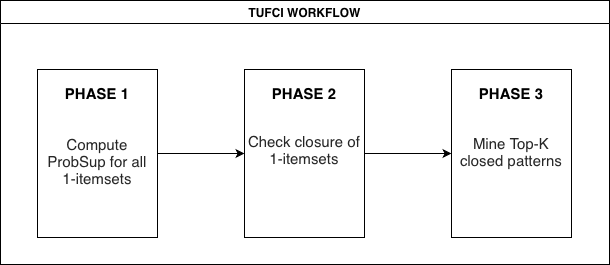
\includegraphics[width=0.85\columnwidth]{images/tufci_workflow.png}
\caption{\textbf{TUFCI framework architecture.}
The algorithm operates in three phases: (1) computing frequent 1-itemsets from the vertical database, (2) initializing data structures and seeding the priority queue, and (3) best-first mining with support-ordered closure verification. The priority queue ensures candidates are processed in descending support order, enabling early termination when the best candidate falls below the dynamic threshold.}
\label{fig:framework}
\end{figure}

Algorithm~\ref{alg:overview} outlines the high-level execution flow of the framework.
\begin{algorithm}[!h]
\caption{TUFCI Framework Overview}
\label{alg:overview}
\begin{algorithmic}[1]
\REQUIRE Uncertain database $\mathcal{D}$, parameter $k$
\ENSURE Top-$k$ closed frequent itemsets $\mathcal{R}$

\STATE \textbf{Phase 1: Preprocessing}
\STATE Scan $\mathcal{D}$ to compute probabilistic support of all 1-itemsets
\STATE Prune items with support $< \$\theta(\mathcal{H})$$

\STATE \textbf{Phase 2: Initialization}
\STATE Initialize candidate structure $\mathcal{Q}$ and result set $\mathcal{R}$
\STATE Seed $\mathcal{Q}$ with frequent 1-itemsets
\STATE Initialize dynamic threshold $\sigma \leftarrow 0$

\STATE \textbf{Phase 3: Mining}
\STATE \textbf{while} $\mathcal{Q}$ is not empty \textbf{do}
\STATE \quad $X \leftarrow ExtractBest(\mathcal{Q})$
\STATE \quad \textbf{if} $support(X) < \sigma$ \textbf{then break}
\STATE \quad Process $X$ and generate extensions
\STATE \textbf{end while}

\RETURN $\mathcal{R}$
\end{algorithmic}
\end{algorithm}


As shown in Algorithm~\ref{alg:overview}, the framework operates in three distinct phases:

\textbf{Phase 1: Preprocessing (Lines 1-3).} 
The algorithm scans the uncertain database to identify frequent 1-itemsets. Items with maximum possible support (tidset size) below the user threshold are globally pruned to reduce the search space dimension.

\textbf{Phase 2: Initialization (Lines 4-6).} 
Data structures are initialized. The Result Heap $\mathcal{R}$ maintains the current top-$k$ patterns, while the Priority Queue $\mathcal{Q}$ orders candidates. The queue is seeded with frequent 1-itemsets, setting the stage for the traversal.

\textbf{Phase 3: Best-First Mining (Lines 7-16).} 
This is the core iterative process. In each step, TUFCI extracts the highest-support candidate $X$. Crucially, if $support(X)$ is lower than the current dynamic threshold $\sigma$, the algorithm terminates immediately (Line 10), as no remaining candidate can qualify. Otherwise, closure is verified, results are updated, and valid extensions are generated for future processing.

\subsection*{Core Mining Components}

The TUFCI algorithm is built upon three core components that enable best-first traversal of the itemset search space: a candidate priority ordering, a dynamic pruning threshold, and a probabilistic vertical data representation. These components are specifically designed to address limitations inherent to depth-first traversal, where candidates are explored according to a fixed enumeration order that is independent of their probabilistic support.

\subsubsection*{Candidate Priority Ordering}

Depth-first search expands itemsets according to a predefined lexicographic order, which does not reflect their probabilistic relevance to the top-{k} objective. As a consequence, itemsets with high probabilistic support may be discovered late in the traversal, delaying threshold updates and weakening pruning effectiveness. In contrast, best-first traversal requires a strict ordering that prioritizes candidates with larger support values.

\begin{definition}[Candidate Priority Order]
\label{def:priority_order}
For two candidate itemsets $X$ and $Y$, $X \succ Y$ ($X$ has higher priority than $Y$) if:
\begin{enumerate}
    \item $\mathit{support}(X) > \mathit{support}(Y)$; or
    \item $\mathit{support}(X) = \mathit{support}(Y)$ and $F_X(S_X) > F_Y(S_Y)$; or
    \item $\mathit{support}(X) = \mathit{support}(Y)$, $F_X(S_X) = F_Y(S_Y)$, and $|X| < |Y|$.
\end{enumerate}
\end{definition}

This ordering ensures that the search always expands the node with the highest potential first, which is the necessary condition for the \textit{Safe Early Termination} property.

\subsubsection*{Dynamic Pruning Threshold}

Unlike traditional mining where the threshold is static, TUFCI maintains a dynamic threshold $\sigma$ derived from the current set of top-$k$ closed patterns found so far.

\begin{definition}[Dynamic Threshold]
Let $\mathcal{R}$ be the current set of $k$ closed frequent itemsets found. The dynamic threshold $\sigma$ is defined as the minimum support in $\mathcal{R}$:
\begin{equation}
\sigma = \begin{cases} 
0 & \text{if } |\mathcal{R}| < k \\
\min_{X \in \mathcal{R}} (\mathit{support}(X)) & \text{if } |\mathcal{R}| = k
\end{cases}
\end{equation}
\end{definition}
The threshold $\sigma$ is a lower bound on the support of any itemset that may belong to the top-k result set. By the anti-monotonicity of probabilistic support, any candidate $X$ such that
$\mathit{support}(X) < \sigma $ and all of its supersets can be pruned. Under best-first traversal, high-support itemsets are examined early, causing $\sigma$ to increase sooner than under depth-first traversal and strengthening pruning effectiveness.


\subsubsection*{Probabilistic Tidset}
\label{subsubsec:ptidset}

To support the rapid support calculations required by the priority queue, we employ a vertical data representation that encapsulates the uncertainty of item occurrences.

\begin{definition}[Probabilistic Tidset]
\label{def:ptidset}
For an itemset $X$, the probabilistic tidset is defined as:
\begin{equation}
\mathit{tidset}(X) = \{(T_j, P(X, T_j)) : T_j \in \mathcal{D}, P(X, T_j) > 0\}
\end{equation}
where $P(X, T_j) = \prod_{i \in X} P(i, T_j)$ assumes independence between items.
\end{definition}

This representation enables efficient support computation and candidate extension via set intersections.

\begin{example}
\label{ex:vertical_db}
Consider the uncertain database in Table~\ref{tab:uncertain_db}. The corresponding vertical database maps each item to its probabilistic tidset.

\begin{table}[!ht]
\caption{\bf Vertical representation of the uncertain database.}
\label{tab:vertical_db}
\centering
\begin{tabular}{c l}
\hline
\textbf{Item $i$} & $\mathit{tidset}(\{i\})$ \\
\hline
$A$ & $\{(T_1,0.9),(T_2,0.8),(T_3,0.9),(T_5,0.7)\}$ \\
$B$ & $\{(T_1,0.8),(T_2,0.7),(T_4,0.8),(T_5,0.6)\}$ \\
$C$ & $\{(T_1,0.7),(T_3,0.8),(T_4,0.9),(T_5,0.8)\}$ \\
$D$ & $\{(T_2,0.6),(T_3,0.7),(T_5,0.9)\}$ \\
$E$ & $\{(T_4,0.5)\}$ \\
\hline
\end{tabular}
\end{table}

Thus, the vertical database $V$ is defined by $V(i)=\mathit{tidset}(\{i\})$ for each item $i\in\mathcal{I}$.
\end{example}

\subsubsection*{Priority Queue and Result Heap}

The priority queue $\mathcal{Q}$ maintains candidate itemsets ordered according to the \textbf{Candidate Priority Order} (Definition~\ref{def:priority_order}). This ordering guarantees that, at each iteration, the candidate with the largest probabilistic support is selected for expansion. 

The result set $\mathcal{R}$ is implemented as a min-heap of fixed size $k$, ordered by probabilistic support. This structure provides constant-time access to the smallest support value among the current top-$k$ patterns. When $|\mathcal{R}| = k$, this minimum value defines the dynamic threshold $\sigma$, which is used for pruning and early termination.


\subsection*{Probabilistic Support Evaluation}
\label{subsec:support_computation}

In TUFCI, the support of a candidate itemset $X$ is a random variable $S_X$ representing the number of transactions in which $X$ occurs. Assuming independence of item existence events across and within transactions, each transaction contributes a Bernoulli trial with probability $p_j = P(X,T_j)$, where $P(X,T_j)=\prod_{i\in X}P(i,T_j)$. Under this assumption, $S_X$ follows a Poisson Binomial distribution.

Let $\sigma$ be the minimum support threshold. To determine whether $X$ is frequent, we compute
\[
P(S_X \ge \sigma) = \sum_{k=\sigma}^{n} D_n[k],
\]
where $D_n[k]=P(S_X=k)$.

TUFCI computes the distribution $\{D_n[k]\}_{k=0}^{n}$ using a \textbf{Direct Convolution} dynamic programming method. For probabilities $P=[p_1,p_2,\ldots,p_n]$, let $D_i[k]$ denote the probability that the support equals $k$ after processing the first $i$ transactions. The recurrence is:
\begin{equation}
D_i[k] = D_{i-1}[k]\cdot(1-p_i) + D_{i-1}[k-1]\cdot p_i,
\end{equation}
with $D_0[0]=1$ and $D_0[k]=0$ for $k>0$.

Algorithm~\ref{alg:direct_conv} computes this distribution in $O(n^2)$ time, where $n$ is the tidset size of $X$. Exact support values are required to correctly order candidates in the priority queue and to enable effective pruning and early termination under the best-first search strategy.



\begin{algorithm}[!h]
\caption{DirectConvolutionSupport}
\label{alg:direct_conv}
\begin{algorithmic}[1]
\small
\REQUIRE List of probabilities $P = [p_1, p_2, \ldots, p_n]$
\ENSURE Support distribution vector $D$ (where $D[k] = P(S_X=k)$)

\STATE Initialize array $D$ of size $n+1$ with zeros
\STATE $D[0] \leftarrow 1.0$ \COMMENT{Probability of support 0 is initially 1}

\FORALL{$p \in P$}
    \FOR{$j$ from $n$ down to $1$}
        \STATE $D[j] \leftarrow D[j] \cdot (1 - p) + D[j-1] \cdot p$
    \ENDFOR
    \STATE $D[0] \leftarrow D[0] \cdot (1 - p)$
\ENDFOR

\RETURN $D$
\end{algorithmic}
\end{algorithm}

\subsection*{Support-ordered closure verification}
\label{subsec:closure_verification}

Closure verification determines whether an itemset $X$ is closed by checking if any of its immediate supersets have the same probabilistic support. In depth-first traversal, extensions are typically examined in a fixed enumeration order that is independent of their support values, which may result in redundant support computations before a closure violation is detected. TUFCI instead evaluates 1-extensions in non-increasing order of support and terminates the check as soon as no remaining extension can match the support of $X$.

The method relies on the anti-monotonicity of probabilistic support with respect to itemset inclusion and on ordering extensions by their support values.

\begin{theorem}[Support-ordered closure verification]
\label{thm:closure}
Let $X$ be an itemset with support $s_X$, and let 
\[
E = \{X \cup \{i_1\}, X \cup \{i_2\}, \ldots, X \cup \{i_m\}\}
\]
be the set of its 1-extensions sorted in non-increasing order of support. If $\mathit{support}(X \cup \{i_j\}) < s_X$ for some index $j$, then for all $\ell > j$ it holds that
\[
\mathit{support}(X \cup \{i_\ell\}) < s_X .
\]
\end{theorem}

\begin{proof}
Because the extensions are sorted in non-increasing order of support, for any $\ell > j$ we have
\[
\mathit{support}(X \cup \{i_\ell\}) \le \mathit{support}(X \cup \{i_j\}) .
\]
If $\mathit{support}(X \cup \{i_j\}) < s_X$, then $\mathit{support}(X \cup \{i_\ell\}) < s_X$ for all $\ell > j$. Hence, once an extension with support strictly smaller than $s_X$ is encountered, no subsequent extension can have support equal to $s_X$, and the closure check can terminate.
\end{proof}


Algorithm~\ref{alg:closure-check} implements this strategy. It first generates candidate 1-extensions and applies inexpensive pruning rules to eliminate extensions that cannot reach the current dynamic threshold. Exact probabilistic support is computed only for the remaining candidates. These candidates are then sorted by support in descending order and examined for closure with early termination based on Theorem~\ref{thm:closure}.

\begin{algorithm}[!h]
\caption{SupportOrderedClosureCheck}
\label{alg:closure-check}
\begin{algorithmic}[1]
\REQUIRE itemset $X$ with $support_X$ and $tidset_X$, extension items $E=\{i: i>\max(X)\}$, dynamic threshold $\sigma$, probability threshold $\tau$
\ENSURE $(isClosed,\, extensions)$
\STATE $extensions \leftarrow \emptyset$
\FORALL{$i \in E$}
    \STATE $Y \leftarrow X \cup \{i\}$
    \IF{$support(\{i\}) < \sigma$} \textbf{continue} \ENDIF
    \STATE $tidset_Y \leftarrow tidset_X \cap tidset(\{i\})$
    \IF{$|tidset_Y| < \sigma$} \textbf{continue} \ENDIF
    \STATE $support_Y \leftarrow ComputeProbabilisticSupport(tidset_Y,\tau)$
    \IF{$support_Y \ge \sigma$}
        \STATE add $(i, support_Y, tidset_Y)$ to $extensions$
    \ENDIF
\ENDFOR
\STATE sort $extensions$ by $support_Y$ in descending order
\FORALL{$(i, support_Y, tidset_Y) \in extensions$}
    \IF{$support_Y = support_X$}
        \RETURN (FALSE, $extensions$) \COMMENT{$X$ is not closed}
    \ELSIF{$support_Y < support_X$}
        \STATE \textbf{break}
    \ENDIF
\ENDFOR
\RETURN (TRUE, $extensions$)
\end{algorithmic}
\end{algorithm}

Processing extensions in support order ensures that if a closure-violating superset exists, it will be encountered before any lower-support extension. This reduces the number of support evaluations required for closure verification. Because best-first traversal maintains a global ordering of candidates by support, it increases the likelihood that high-support extensions are generated and checked earlier than under depth-first traversal, which explores candidates according to a fixed structural order. Consequently, support-ordered closure verification complements the best-first search strategy and contributes to reducing redundant computations in TUFCI.
\subsection*{Best-first search with early termination}

\subsubsection*{Rationale for the search strategy}

Traditional itemset mining algorithms typically employ Depth-First Search (DFS) to traverse the search space. While DFS uses memory efficiently, it traverses candidates in a predetermined structural order that is independent of their probabilistic support values. As a result, itemsets with high probabilistic support—whose early discovery is critical for elevating the dynamic threshold \(\sigma\)—may be encountered late in the traversal. This delay can keep \(\sigma\) low over much of the search and reduce the effectiveness of pruning.

In contrast, TUFCI adopts a Best-First Search (BFS) strategy based on the priority queue. By always selecting the candidate with the highest probabilistic support for expansion, the algorithm tends to discover high-support itemsets early. Early updates to the dynamic threshold \(\sigma\) strengthen pruning conditions and reduce exploration of low-support regions of the search space.

\subsubsection*{Early termination condition}

An important property of the BFS strategy is that it enables safe early termination of the search based on the current dynamic threshold.

\begin{lemma}[Early termination]
\label{lemma:early-term}
Let \(\mathcal{Q}\) be a priority queue ordered by non-increasing probabilistic support, and let \(\sigma\) denote the current minimum support among the top-\(k\) closed itemsets found so far. If the head of \(\mathcal{Q}\), denoted \(X\), satisfies \(\mathit{support}(X) < \sigma\), then the search can terminate without further exploration.
\end{lemma}

\begin{proof}
Since \(\mathcal{Q}\) is ordered by non-increasing support, if the maximum-support candidate \(X\) has \(\mathit{support}(X) < \sigma\), then all remaining candidates \(Y \in \mathcal{Q}\) must satisfy \(\mathit{support}(Y) \le \mathit{support}(X) < \sigma\). By the pruning correctness result, no candidate with support less than \(\sigma\) can belong to the top-\(k\) result set. Therefore, none of the remaining candidates can improve the result set, and the search can terminate safely.
\end{proof}

\begin{figure}[!ht]
    \centering
    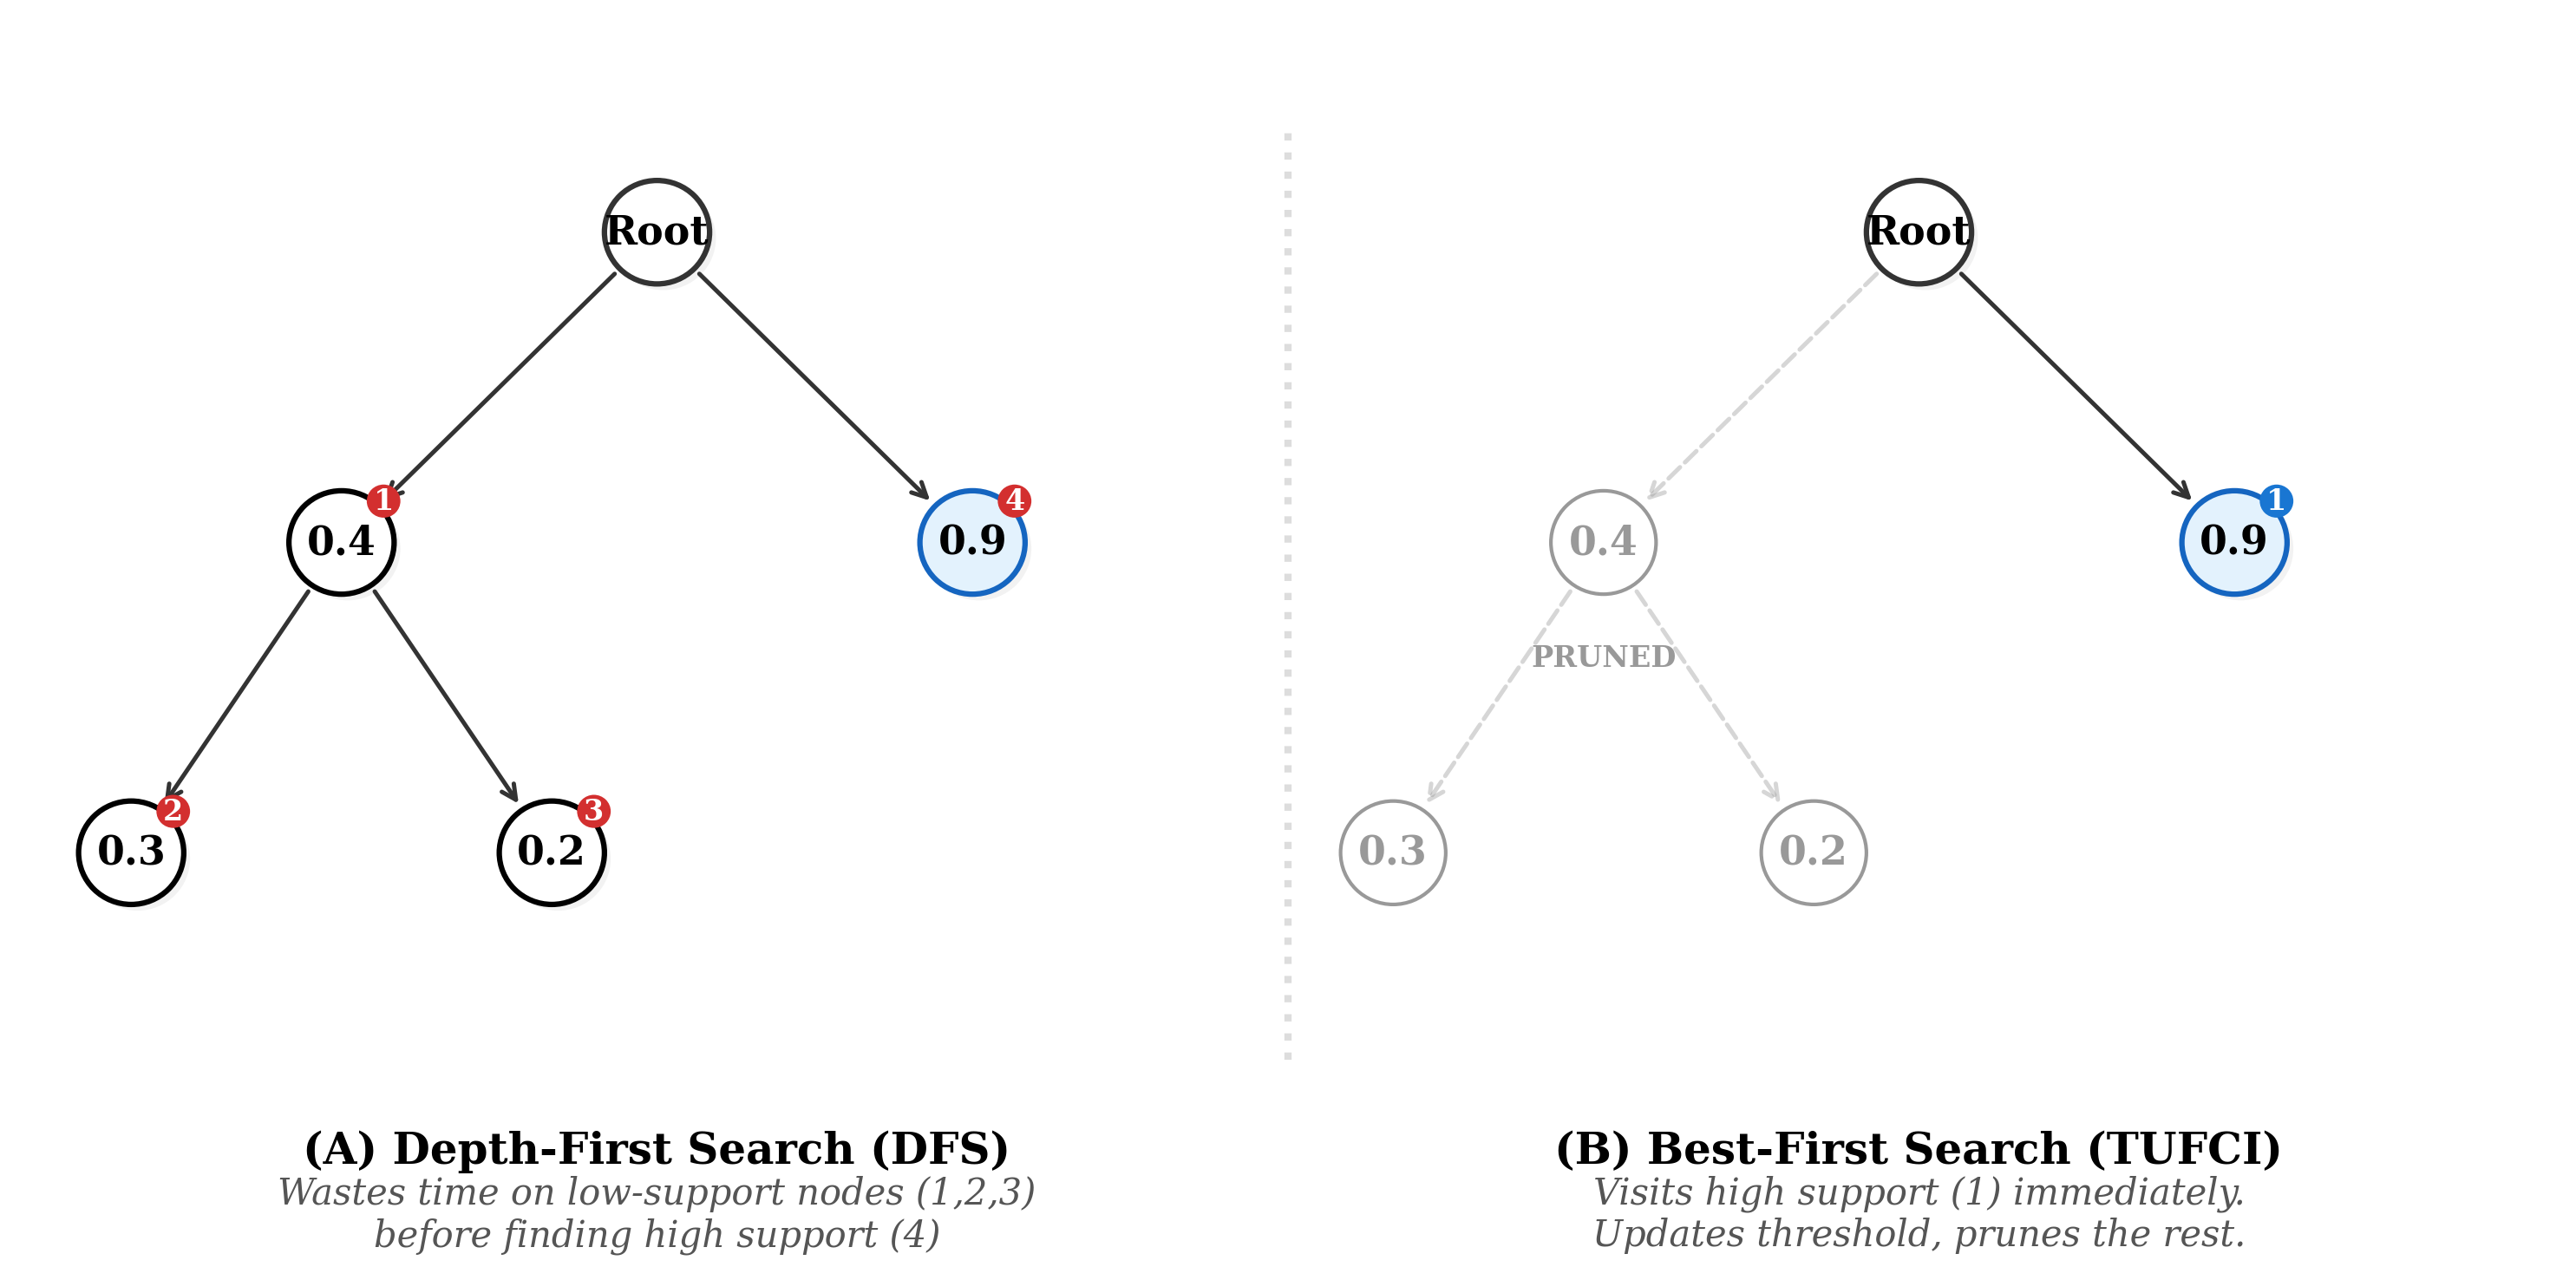
\includegraphics[width=0.95\columnwidth]{images/DFS_BFS_Comparision.png}
    \caption{\textbf{Traversal order comparison.} (A) Under DFS, exploration proceeds according to structural order. (B) Under best-first search, candidates with higher support are visited first, which can lead to earlier threshold updates and pruning.}
    \label{fig:comparison}
\end{figure}

Figure~\ref{fig:comparison} illustrates this difference in traversal behavior. In the DFS case (A), exploration may proceed deep into branches with low support before reaching high-support itemsets. In the Best-First Search case (B), the highest-support itemsets are visited first, and \(\sigma\) can be updated early, enabling the remaining low-support candidates to be pruned without further expansion.



\subsection*{The TUFCI Algorithm}

The TUFCI framework is architected into three distinct phases to efficiently handle the complexity of uncertain data mining. By decoupling preprocessing, initialization, and the core mining loop, the algorithm maximizes modularity and allows for specific optimizations at each stage.

\subsubsection*{Phase 1: Preprocessing and Frequent 1-Itemset Generation}
The first phase (Algorithm~\ref{alg:phase1}) is responsible for transforming the raw data into a structure suitable for efficient intersection. It converts the horizontal uncertain database into a vertical format (tidsets). 

Crucially, it computes the exact probabilistic support for all single items using the convolution method. Items that fail to meet the minimum support threshold $\sigma$ are pruned immediately. The remaining items are sorted in descending order of support. This sorting is the foundation of the \textit{Best-First} strategy, ensuring that the search tree is explored starting from the most promising branches.

\begin{algorithm}[H]
\caption{Phase 1: Preprocessing}
\label{alg:phase1}
\begin{algorithmic}[1]
\footnotesize
\REQUIRE Uncertain database $\mathcal{D}$, min support $\sigma$, threshold $\tau$
\ENSURE Sorted list of frequent 1-itemsets $\mathcal{F}_1$

\STATE $V \leftarrow buildVerticalDatabase(\mathcal{D})$
\STATE $\mathcal{F}_1 \leftarrow$ empty list
\FORALL{item $i \in \mathcal{I}$} 
    \STATE $tidset\_i \leftarrow V.getTidset(i)$
    \IF{$tidset\_i$ is empty} \STATE \textbf{continue} \ENDIF
    \STATE $(support\_i, prob\_i) \leftarrow ComputeProbabilisticSupport(tidset\_i, \tau)$
    \IF{$support\_i \geq \sigma$}
        \STATE $\mathcal{F}_1.add(\{i\}, support\_i, prob\_i, tidset\_i)$
    \ENDIF
\ENDFOR
\STATE Sort $\mathcal{F}_1$ by support descending
\RETURN $\mathcal{F}_1$
\end{algorithmic}
\end{algorithm}

\subsubsection*{Phase 2: Initialization}
In the second phase (Algorithm~\ref{alg:phase2}), we initialize the core data structures: the \textbf{Top-$k$ Heap} ($\mathcal{R}$) to store the current best closed itemsets, and the \textbf{Max-Priority Queue} ($\mathcal{Q}$) to manage the search frontier. 

The Priority Queue is seeded with the frequent 1-itemsets identified in Phase 1. A preliminary closure check is performed here: if a 1-itemset is already subsumed by a superset (formed with items appearing later in the sort order) that has the same support, it is not added to the results as a closed candidate, though it remains available for extension generation.

\begin{algorithm}[H]
\caption{Phase 2: Initialization}
\label{alg:phase2}
\begin{algorithmic}[1]
\footnotesize
\REQUIRE Sorted frequent 1-itemsets $\mathcal{F}_1$, integer $k$, initial $\sigma$
\ENSURE Priority Queue $\mathcal{Q}$, Result Heap $\mathcal{R}$, dynamic threshold $\sigma$

\STATE $\mathcal{R} \leftarrow MinHeap(k)$ \COMMENT{Stores top-k results}
\STATE $\mathcal{Q} \leftarrow MaxPriorityQueue()$ \COMMENT{Ordered by support desc}
\STATE $\sigma \leftarrow \sigma$

\STATE \textit{// Seed priority queue with closed 1-itemsets}
\FORALL{$(\{i\}, support\_i, prob\_i, tidset\_i) \in \mathcal{F}_1$}
    \STATE $E \leftarrow \{j : j > i \text{ and } support(\{j\}) \geq \sigma\}$
    \STATE $(isClosed, \_) \leftarrow SupportOrderedClosureCheck(\{i\}, E, \sigma, \tau)$
    
    \IF{$isClosed$ \AND $support\_i \geq \sigma$}
        \STATE $\mathcal{Q}.insert(\{i\}, support\_i, prob\_i, tidset\_i)$
    \ENDIF
\ENDFOR
\RETURN $(\mathcal{Q}, \mathcal{R}, \sigma)$
\end{algorithmic}
\end{algorithm}

\subsubsection*{Phase 3: Best-First Mining Process}
The core mining loop is presented in Algorithm~\ref{alg:phase3}. This phase iteratively extracts the candidate with the highest support from $\mathcal{Q}$ and performs three critical operations:
\begin{enumerate}
    \item \textbf{Early Termination:} If the support of the extracted candidate is less than the current dynamic threshold $\sigma$, the algorithm terminates immediately. Since $\mathcal{Q}$ is sorted, no remaining candidate can possibly qualify for the top-$k$ set (Lemma 3).
    \item \textbf{Expansion \& Closure:} The candidate is expanded to generate supersets. We simultaneously check if the candidate is closed.
    \item \textbf{Result Update:} If closed, it is added to $\mathcal{R}$. If $\mathcal{R}$ becomes full, $\sigma$ is raised to the support of the $k$-th best pattern, effectively pruning the remaining search space.
\end{enumerate}

\begin{algorithm}[H]
\caption{Phase 3: Best-First Mining}
\label{alg:phase3}
\begin{algorithmic}[1]
\footnotesize
\REQUIRE Queue $\mathcal{Q}$, Heap $\mathcal{R}$, threshold $\sigma$, $k$, $\tau$
\ENSURE Final Top-$k$ closed frequent itemsets $\mathcal{R}$

\WHILE{$\mathcal{Q}$ is not empty}
    \STATE $(X, support\_X, prob\_X, tidset\_X) \leftarrow \mathcal{Q}.extractMax()$
    
    \STATE \textit{// 1. Global Pruning / Early Termination}
    \IF{$support\_X < \sigma$} 
        \STATE \textbf{break} \COMMENT{Safe to stop: all subsequent candidates have lower support}
    \ENDIF
    
    \STATE \textit{// 2. Generate Extensions \& Check Closure}
    \STATE $E \leftarrow \{i : i > \max(X) \text{ and } support(\{i\}) \geq \sigma\}$
    \STATE $(isClosed, extensions) \leftarrow SupportOrderedClosureCheck(X, E, \sigma, \tau)$
    
    \STATE \textit{// 3. Update Top-K Results}
    \IF{$isClosed$}
        \STATE $\mathcal{R}.insert(X, support\_X)$
        \IF{$|\mathcal{R}| > k$} \STATE $\mathcal{R}.removeMin()$ \ENDIF
        \IF{$|\mathcal{R}| = k$} \STATE $\sigma \leftarrow \max(\sigma, \mathcal{R}.peekMin().support)$ \ENDIF
    \ENDIF
    
    \STATE \textit{// 4. Expand Search Space}
    \FORALL{$(i, support\_Y, prob\_Y, tidset\_Y) \in extensions$}
        \IF{$support\_Y \geq \sigma$}
            \STATE $\mathcal{Q}.insert(X \cup \{i\}, support\_Y, prob\_Y, tidset\_Y)$
        \ENDIF
    \ENDFOR
\ENDWHILE
\RETURN $\mathcal{R}$
\end{algorithmic}
\end{algorithm}

\subsubsection*{Execution Walkthrough with Example}
To clarify the interaction between these phases, consider the uncertain database from Table~\ref{tab:uncertain_db} with threshold $\tau=0.7$ and $k=2$.

\textbf{Phase 1 (Preprocessing):} 
Items are evaluated. Suppose the computed probabilistic supports are: $A=3, C=3, B=2, D=2$.
Sorted $\mathcal{F}_1 = \langle A, C, B, D \rangle$.

\textbf{Phase 2 (Initialization):} 
Priority Queue $\mathcal{Q}$ is seeded with the frequent 1-itemsets.
\begin{equation}
\mathcal{Q} = [ (A, 3), (C, 3), (B, 2), (D, 2) ]
\end{equation}
Result heap $\mathcal{R}$ is empty; $\sigma = 0$.

\textbf{Phase 3 (Mining):}
\begin{itemize}
    \item \textbf{Iteration 1:} Extract $A$ (support 3). Check extensions ($AB, AC$). Assume extensions have support 2. Since $sup(A) > sup(extensions)$, $A$ is \textbf{Closed}. 
    \begin{itemize}
        \item Add $A$ to $\mathcal{R}$. Top-$k$: $\{A\}$.
        \item Add $AB, AC$ to $\mathcal{Q}$.
    \end{itemize}
    \item \textbf{Iteration 2:} Extract $C$ (support 3). Assume $C$ is closed.
    \begin{itemize}
        \item Add $C$ to $\mathcal{R}$. Top-$k$: $\{A, C\}$.
        \item \textbf{Update $\sigma$:} $\mathcal{R}$ is full ($k=2$). Minimum support in $\mathcal{R}$ is 3. New $\sigma = 3$.
    \end{itemize}
    \item \textbf{Iteration 3:} Extract next best candidate (e.g., $B$ or $AB$, which have support 2).
    \item \textbf{Termination Check:} Current candidate support (2) $< \sigma$ (3). 
    \item \textbf{Action:} Algorithm breaks immediately.
\end{itemize}
This demonstrates how TUFCI avoids processing low-support patterns ($B, D, \dots$) entirely once the Top-$k$ buffer is filled with high-quality patterns.


\subsection*{Pruning Strategies}
\label{subsec:pruning}

To address the exponential search space inherent in uncertain databases, TUFCI integrates seven distinct pruning strategies (P1–P7). These strategies are applied hierarchically, prioritizing low-cost checks ($O(1)$ or $O(N)$) to eliminate unpromising candidates before invoking the computationally expensive convolution algorithm ($O(N^2)$).

\subsubsection*{Strategy 1: Early Termination (P1)}
This strategy, unique to the Best-First approach, serves as the most critical pruning mechanism for sparse datasets. Since the priority queue $\mathcal{Q}$ orders candidates by support, if the head of the queue falls below the threshold $\sigma$, the search terminates immediately.
\begin{equation}
\text{If } \mathcal{Q}.\mathit{peek}().support < \sigma \Rightarrow \text{Terminate Global Search}
\end{equation}

\subsubsection*{Strategy 2: Dynamic Threshold Pruning (P2)}
As the mining progresses and $k$ patterns are discovered, the internal threshold $\sigma$ rises. By Lemma~\ref{lem:antimonotonicity}, any candidate $X$ generated with $\mathit{ProbSup}(X) < \sigma$ is immediately discarded, preventing the generation of its supersets.

\subsubsection*{Strategy 3: Item-Level Filtering (P3)}
In Phase 1, we filter 1-itemsets based on exact probabilistic support. Any item $i$ where $\mathit{ProbSup}(\{i\}) < \sigma$ is permanently removed from the database.
\begin{equation}
\mathcal{D}' = \mathcal{D} \setminus \{i \in \mathcal{I} : \mathit{ProbSup}(\{i\}) < \sigma\}
\end{equation}
This strategy effectively reduces the width of the lattice and provides consistent performance gains across dense datasets.

\subsubsection*{Strategy 4: Transaction Trimming (P4)}
After global item filtering, transactions that contain fewer items than the minimum pattern length (or become empty) are removed. Additionally, transactions with very low existence probabilities that cannot mathematically contribute to reaching $\sigma$ are trimmed to compress the vertical database.

\subsubsection*{Strategy 5: Expected Support Upper Bound (P5)}
Before computing the exact probabilistic support distribution, we calculate the \textit{Expected Support} ($E[S_X]$), which is the sum of existence probabilities.
\begin{equation}
E[S_X] = \sum_{t \in \mathit{tidset}(X)} P(X \in t)
\end{equation}
Since $ProbSup(X) \leq E[S_X]$, if $E[S_X] < \sigma$, the candidate is pruned. This $O(N)$ check is significantly faster than the $O(N^2)$ exact calculation.

\subsubsection*{Strategy 6: Tidset Intersection Look-ahead (P6)}
When expanding a candidate $X$ with item $i$, we compute the size of the intersection of their tidsets $|\mathit{tidset}(X) \cap \mathit{tidset}(\{i\})|$ before generating the new node.
\begin{equation}
\text{If } |\mathit{tidset}(X) \cap \mathit{tidset}(\{i\})| < \sigma \Rightarrow \text{Prune extension } X \cup \{i\}
\end{equation}
While highly effective for sparse data, this strategy is applied conditionally, as the intersection overhead can outweigh the benefits in very dense datasets.

\subsubsection*{Strategy 7: Closure Optimization (P7)}
TUFCI leverages the closure property to reduce redundant processing. If a candidate $X$ is found to be non-closed (i.e., $\exists Y \supset X$ such that $Sup(Y) = Sup(X)$), $X$ is marked. If $X$ is fully subsumed by a previously processed closed pattern, its extensions are skipped under specific canonical ordering conditions, ensuring minimal redundancy.

\begin{theorem}[Pruning Correctness]
\label{thm:pruning}
The pruning strategies P1–P7 do not eliminate any true top-$k$ closed frequent itemset.
\end{theorem}

\begin{proof}
All strategies rely on the anti-monotonicity of valid upper bounds. P1 and P2 strictly enforce the minimal support definition. P3, P4, P5, and P6 utilize mathematically proven upper bounds ($Cardinality \ge Expected \ge Probabilistic$); if an upper bound is below $\sigma$, the true support must also be below $\sigma$. P7 ensures only non-closed (redundant) or subsumed branches are pruned, preserving the set of Closed Frequent Itemsets.
\end{proof}




% Results and Discussion can be combined.
\section*{Performance evaluation}

\subsection*{Dataset Synthesis and Uncertainty Generation}

Since standard benchmark datasets from the SPMF repository are deterministic, we generated uncertain databases using a synthetic injection method consistent with experimental protocols in probabilistic frequent itemset mining literature. The transformation follows the tuple-independent model, where every item occurrence is associated with an independent existence probability.

To ensure realistic data characteristics, we employed a three-stage generation process (Random Seed = 42):

\begin{enumerate}
    \item \textbf{Support-Correlated Probability:} We reflect the real-world observation that frequent items often have higher data quality. The base probability $P_{base}(i)$ for an item $i$ is assigned proportional to its normalized frequency $f(i)$:
    \begin{equation}
        P_{base}(i) = P_{min} + (P_{max} - P_{min}) \times f(i)^\alpha
    \end{equation}
    where $P_{min}=0.1$, $P_{max}=1.0$, and the skew exponent $\alpha=1.0$.

    \item \textbf{Transaction Length Adaptation:} To simulate sensor noise where larger transactions are more prone to errors, we apply a penalty factor to transactions exceeding the average length $\mu_{len}$:
    \begin{equation}
        P_{final}(i, T) = P_{base}(i) \times \left(1 - 0.5 \times \frac{\max(0, |T| - \mu_{len})}{\mu_{len}}\right)
    \end{equation}

    \item \textbf{Noise Injection:} To test robustness, we injected random noise with probability $\rho=0.02$, decoupling specific items from their support and assigning them a random low probability in the range $[0.05, P_{base}]$.
\end{enumerate}

\subsection*{Experimental setup}

\subsubsection*{Datasets}

We selected four real-world datasets representing diverse mining scenarios to evaluate the framework's adaptability:

\begin{itemize}
    \item \textbf{Dense datasets (Chess, Mushroom):} Characterized by a small item universe but high item frequency and strong correlations. These datasets generate long patterns and heavily stress the closure verification and probabilistic support computation components.
    \item \textbf{Sparse datasets (Retail, Liquor):} Characterized by large item universes and variable transaction lengths. These datasets test the algorithm's scalability and the effectiveness of pruning strategies in reducing the search space.
\end{itemize}

The characteristics of the generated uncertain datasets are summarized in Table~\ref{tab:datasets}.

\begin{table}[H]
\centering
\caption{Characteristics of experimental datasets.}
\label{tab:datasets}
\begin{tabular}{lrrrrl}
\hline
\textbf{Dataset} & \textbf{Transactions} & \textbf{Items} & \textbf{Avg. length} & \textbf{Density} \\
\hline
Chess      & 3,197  & 82     & 14.7  & Dense \\
Mushroom   & 8,125  & 119    & 23.0  & Dense \\
Retail     & 88,162 & 16,470 & 10.3  & Sparse \\
Liquor     & 52,819 & 11,039 & 33.0  & Sparse \\
\hline
\end{tabular}
\end{table}

\subsubsection*{Analyzed Variants}

To isolate the effects of search strategy and pruning, four algorithm variants were evaluated (Table~\ref{tab:variants}). Variant V1 implements the proposed TUFCI using best-first search with the full pruning suite. Variant V2 adopts depth-first traversal with the same pruning to assess the impact of search order. Variant V3 uses best-first search with minimal pruning to evaluate pruning effectiveness. Variant V4 is a naive baseline using depth-first traversal with minimal pruning.

\begin{table}[H]
\centering
\caption{Summary of algorithm variants.}
\label{tab:variants}
\begin{tabular}{llll}
\hline
\textbf{Variant} & \textbf{Search strategy} & \textbf{Pruning} & \textbf{Purpose} \\
\hline
V1 & Best-first (PQ) & Full (P1--P7) & Proposed method \\
V2 & Depth-first (stack) & Full (P1--P7) & Search strategy comparison \\
V3 & Best-first (PQ) & Minimal & Pruning impact evaluation \\
V4 & Depth-first (stack) & Minimal & Naive baseline \\
\hline
\end{tabular}
\end{table}

\subsubsection*{Implementation Environment}

All algorithms were implemented in Java (JDK~21) within the TUFCI framework. To ensure fair comparison, all experiments were executed in single-user mode with no other intensive processes running. The experiments were conducted on a workstation with the following specifications:

\begin{itemize}
    \item \textbf{Processor:} Intel Core i7--12700H (2.30~GHz)
    \item \textbf{Memory:} 16~GB DDR4 RAM
    \item \textbf{Operating System:} Windows~11 (64-bit)
\end{itemize}

\subsection*{Experimental Results and Analysis}

We evaluated the performance of TUFCI across three key dimensions: runtime scalability, computational overhead (closure checks), and memory consumption.

\subsubsection*{Runtime Scalability}
Figure~\ref{fig:runtime} illustrates the execution time of the four variants across dense (Chess, Mushroom) and sparse (Retail, Liquor) datasets.

\begin{itemize}
    \item \textbf{Superiority of Best-First Search (V1 vs. V2):} The proposed Best-First strategy (V1) consistently achieved the lowest runtime. On the dense \textbf{Chess} dataset ($k=50$), V1 was approximately \textbf{2$\times$ faster} than the DFS baseline (V2). This gap is attributed to the \textit{Early Termination} property: V1 prioritizes high-probability patterns, rapidly raising the dynamic threshold $\sigma$ to prune low-support branches that DFS is forced to explore.
    \item \textbf{Impact of Pruning (V1 vs. V3):} While Best-First Search alone (V3) is efficient, adding the full pruning suite (V1) provides further gains, particularly on sparse datasets like \textbf{Retail}. V3 suffers from overhead in managing a larger priority queue, whereas V1 uses upper-bound pruning (P4--P6) to prevent unpromising candidates from entering the queue.
    \item \textbf{Inefficiency of Baseline (V4):} The naive DFS variant (V4) exhibited the worst performance across all scenarios, confirming that uncertain frequent itemset mining is computationally infeasible without aggressive pruning and optimized traversal.
\end{itemize}

\begin{figure}[H]
    \centering
    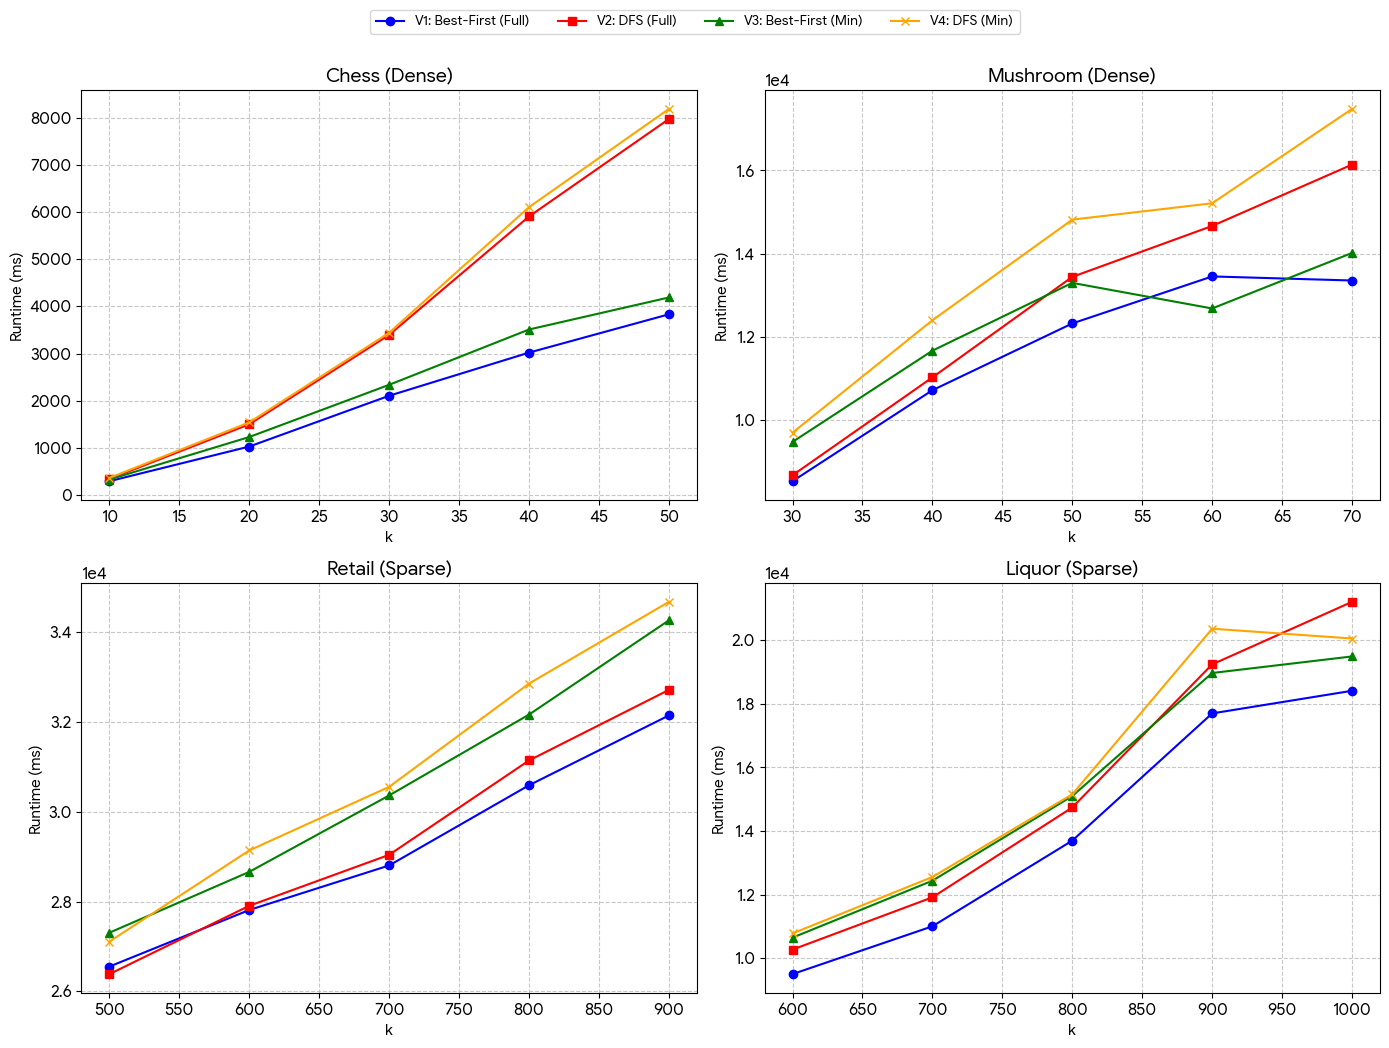
\includegraphics[width=0.95\linewidth]{images/Runtime_Comparison.png}
    \caption{Runtime comparison of TUFCI variants. V1 (Proposed) consistently outperforms DFS variants (V2, V4) and the minimal-pruning baseline (V3).}
    \label{fig:runtime}
\end{figure}

\subsubsection*{Efficiency of Closure Verification}
Closure checking is the most expensive operation in the mining process. Figure~\ref{fig:closure} compares the number of closure checks performed.

\begin{itemize}
    \item \textbf{Search Strategy Dominance:} A key observation is that the variants group by search strategy: V1 mirrors V3, while V2 mirrors V4. This indicates that search order, not pruning, is the primary driver of closure efficiency.
    \item \textbf{Best-First Efficiency (V1 \& V3):} Both Best-First variants identify the top-$k$ patterns early, raising $\sigma$ to its maximum value. Even though V3 lacks advanced pruning, it discards candidates via the $sup(X) < \sigma$ check \textit{before} performing the expensive closure test. Consequently, V1 and V3 perform nearly identical numbers of checks, approximately \textbf{60\% fewer} than the DFS variants on dense data.
    \item \textbf{DFS Redundancy (V2 \& V4):} The rigid traversal of DFS keeps $\sigma$ low for a longer duration, forcing V2 and V4 to verify the closure of thousands of locally valid but globally suboptimal patterns.
\end{itemize}

\begin{figure}[H]
    \centering
    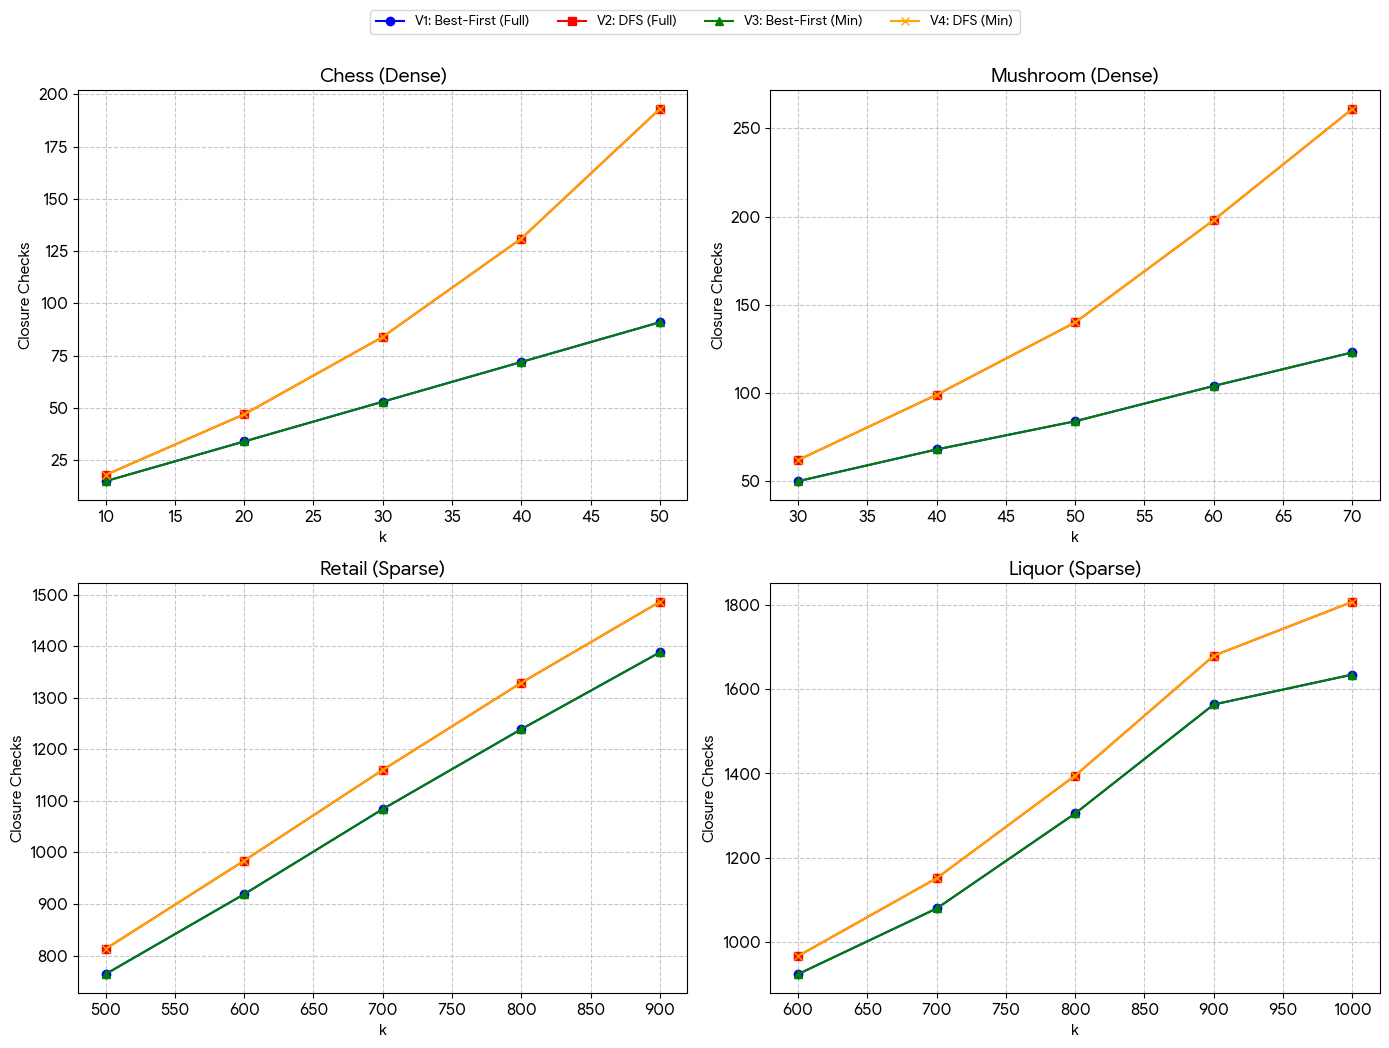
\includegraphics[width=0.95\linewidth]{images/Closure_Checks_Comparison.png}
    \caption{Number of closure verifications. The curves show that Best-First strategies (V1, V3) minimize expensive checks by quickly raising the pruning threshold, whereas DFS (V2, V4) incurs significant overhead.}
    \label{fig:closure}
\end{figure}

\subsubsection*{Memory Consumption}
A common concern with Best-First Search is memory explosion due to the priority queue size. However, Figure~\ref{fig:memory} demonstrates that TUFCI manages memory effectively.

\begin{itemize}
    \item \textbf{Stability of V1:} On dense datasets like \textbf{Mushroom}, V1 maintains a stable memory footprint. The combination of Upper Bound Pruning (P4--P6) and Early Termination (P1) ensures that the priority queue never grows uncontrollably.
    \item \textbf{DFS Stack Explosion:} Surprisingly, the DFS variants (V2, V4) often consumed \textit{more} memory than V1 on dense datasets. This is because DFS gets trapped in deep recursive branches, generating and storing many candidates in the stack before they can be pruned.
\end{itemize}

\begin{figure}[H]
    \centering
    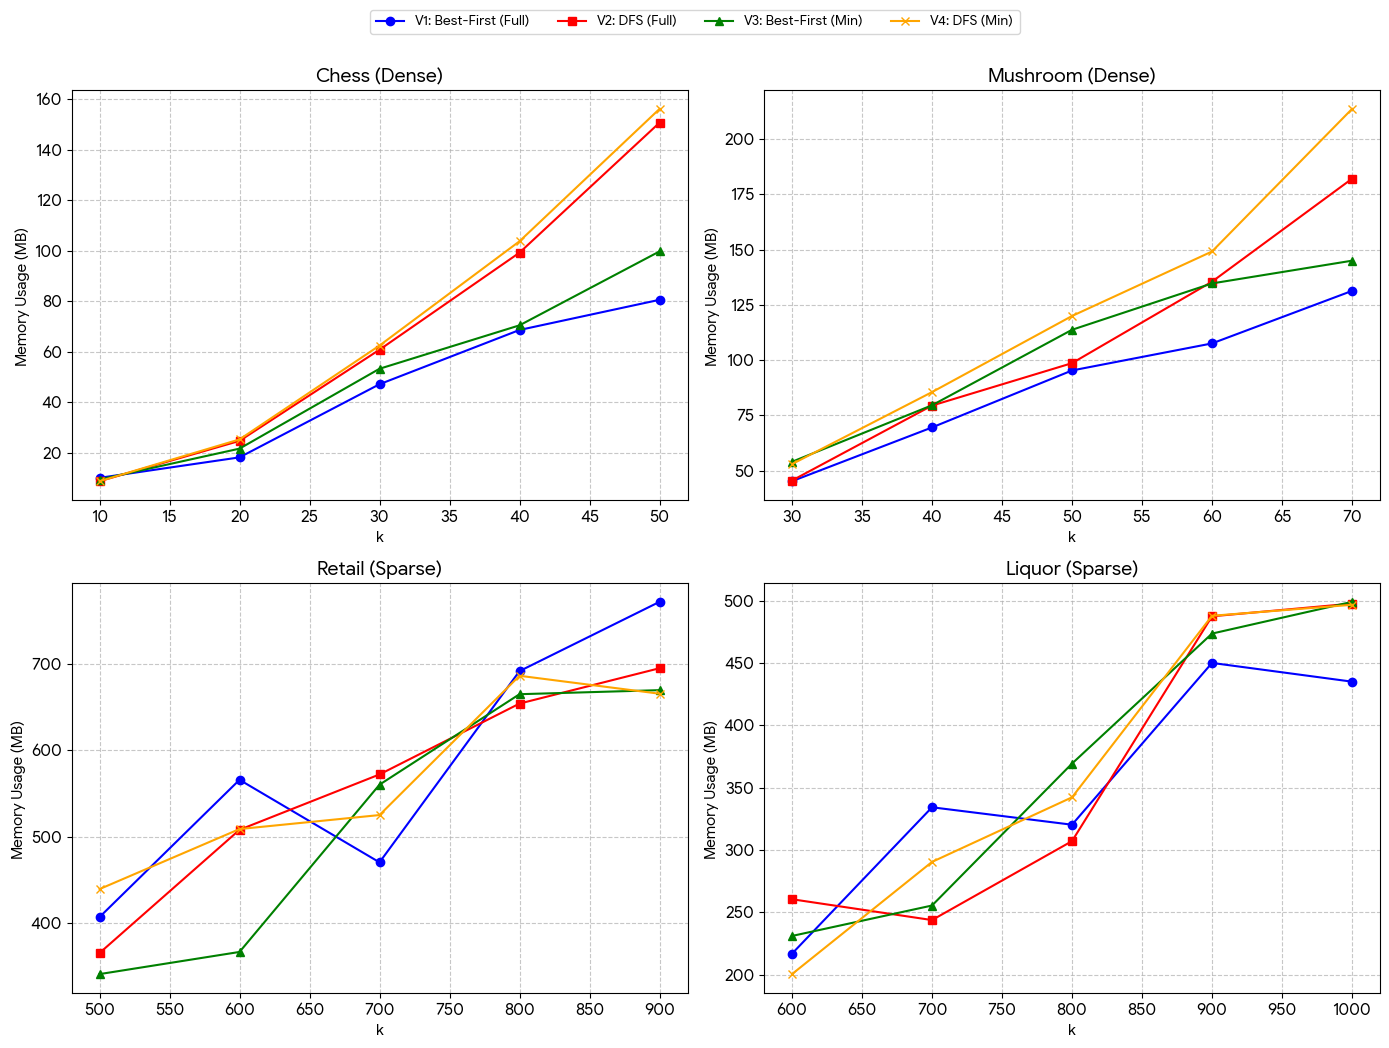
\includegraphics[width=0.95\linewidth]{images/Memory_Usage_Comparison.png}
    \caption{Peak memory usage (MB). V1 remains memory-efficient even on dense datasets, whereas unpruned BFS (V3) and deep DFS (V2) show higher consumption.}
    \label{fig:memory}
\end{figure}

\subsubsection*{Ablation Study}
To quantify the contribution of specific pruning strategies, we conducted an ablation study on the Chess dataset (Table~\ref{tab:ablation}). Strategy \textbf{P1 (Early Termination)} provided the largest individual speedup ($11\%$), followed by \textbf{P7 (Closure Optimization)}. This confirms that dynamic search space reduction is the most vital optimization in the TUFCI framework.

\begin{table}[H]
\centering
\caption{Incremental speedup of Pruning Strategies (Chess, $k=100$).}
\label{tab:ablation}
\begin{tabular}{llcc}
\hline
\textbf{Configuration} & \textbf{Added Strategy} & \textbf{Time (ms)} & \textbf{Speedup} \\
\hline
Base (V3) & Minimal Pruning & 12,351 & 1.00x \\
+ P1 & Early Termination & 11,165 & 1.11x \\
+ P2 & Dynamic Threshold & 11,056 & 1.12x \\
+ P3 & Item Filtering & 9,920 & 1.25x \\
+ P4--P6 & Upper Bounds & 9,787 & 1.26x \\
+ P7 & Closure Optimization & \textbf{9,468} & \textbf{1.30x} \\
\hline
\end{tabular}
\end{table}

\subsection*{Conclusion of Experiments}
The experimental results conclusively demonstrate that TUFCI's architecture—combining \textbf{Best-First Search} and the full suite of \textbf{Pruning Strategies (P1--P7)}—is highly effective. V1 yields the best scalability and runtime performance, successfully addressing the exponential search space of mining top-$k$ closed frequent itemsets in uncertain databases.

\section*{Conclusion}

This paper presented TUFCI, a best-first search algorithm for mining top-$k$ closed frequent itemsets from uncertain databases. Unlike existing depth-first search approaches that explore candidates in enumeration order, TUFCI processes candidates in descending order of probabilistic support using a priority queue. This support-ordered exploration strategy addresses three fundamental limitations of DFS-based methods: delayed discovery of high-support patterns, inefficient closure verification, and inability to terminate early.

The main contributions of this work are summarized as follows. First, we proposed a best-first search framework that aligns the exploration order with the top-$k$ mining objective, ensuring that strong patterns are discovered early and the dynamic pruning threshold rises rapidly. Second, we introduced a support-ordered closure verification strategy that examines supersets in descending support order, enabling early detection of closure violations and reducing redundant support computations. Third, we established a safe early termination condition that allows TUFCI to stop exploration when the best remaining candidate falls below the current threshold, a property that DFS-based approaches cannot exploit. Fourth, we developed multiple pruning strategies specifically designed for best-first traversal, including support-based pruning, upper bound pruning, and item-level filtering.

Experimental results demonstrated that TUFCI significantly outperforms DFS-based approaches in terms of runtime, particularly on dense datasets where the search space is large and pruning effectiveness is critical. The support-ordered closure verification reduced the number of superset examinations by detecting violations early, while the early termination condition allowed TUFCI to avoid exploring large portions of the search space once the top-$k$ patterns were identified. The best-first strategy also exhibited more consistent performance across different dataset characteristics, as the threshold elevation rate is determined by pattern supports rather than enumeration order.

The trade-off of the best-first approach is moderate additional memory consumption for maintaining the priority queue compared to the stack-based memory usage of DFS. However, this overhead is justified by the substantial runtime improvements, especially for applications where mining efficiency is prioritized over memory constraints.

Several directions remain for future work. First, the best-first framework could be extended to other pattern mining problems, including high utility itemset mining and sequential pattern mining, where support-ordered exploration may provide similar benefits. Second, distributed and parallel implementations of TUFCI could be developed to handle large-scale uncertain databases that exceed single-machine capacity. Third, approximate mining techniques could be integrated to further reduce computational cost while providing probabilistic guarantees on result quality. Finally, the interaction between best-first search and other advanced pruning techniques, such as co-occurrence pruning and transaction merging, warrants further investigation to identify optimal combinations for different dataset characteristics.

In conclusion, this work demonstrates that the choice of search strategy significantly impacts the efficiency of top-$k$ closed frequent itemset mining from uncertain databases. By replacing depth-first traversal with best-first exploration, TUFCI achieves substantial performance improvements through early pattern discovery, efficient closure verification, and safe early termination. The proposed approach provides a new perspective on uncertain pattern mining and opens opportunities for applying best-first search to related data mining problems.
\pagebreak
\bibliography{plos_bibtex_sample}

\end{document}


